L'interopérabilité des données, recherchée par les plateformes numériques à l'instar de LaDocumenta.eu, suppose un cadre méthodologique de structuration et de normalisation rigoureuse des données. Appliquée aux bibliothèques spécialisées que représentent les bibliothèques d'orchestre, cette exigence technique est la condition pour que les documents patrimoniaux (conducteurs annotés, matériel d'orchestre, etc.) deviennent des données de recherche exploitables et interopérables pour nourrir l'interprétation historiquement informée. La transformation de ces sources matérielles en ressources interopérables permet dès lors aux musicologues, musiciens et chercheurs de disposer d'outils pour documenter et restituer les pratiques historiquement informées au moyen de portails documentaires interrogeables entre eux. Pour comprendre la portée de cette transformation, il convient d'étudier le passage du signalement traditionnel aux métadonnées structurées pour analyser la capacité des standards du web de données à traiter la complexité des données musicales. Cette démarche correspond à un objectif d'interaction et de réutilisation des données à l'échelle européenne puis internationale.

\subsection*{Du signalement traditionnel aux métadonnées structurées}

En bibliothéconomie, il est d'usage d'élaborer une politique documentaire pour régir la vie de la bibliothèque, que ce soit au niveau de l'organisation ou de la médiation des collections. Dans une plateforme numérique, la politique de gouvernance des données, qui cadre et pilote le traitement de la donnée, remplit le même rôle. Ainsi, on observe une transformation des pratiques en bibliothèques allant d'un signalement traditionnel à une réflexion centrée sur les données.

\subsubsection*{De la fiche bibliographique aux métadonnées structurées : \enquote{La bibliothèque face au monde des données}\footnote{Mesguich (Véronique), \textit{Les bibliothèques face au monde des données}, Presses de l’enssib, 2023, \url{https://doi.org/10.4000/books.pressesenssib.17686}.}}

Comme nous l'avons vu dans le premier chapitre, la transformation numérique des bibliothèques a profondément reconfiguré leurs modes d'accès et leurs supports.

Le signalement — entendu comme \enquote{la description de documents constituant un fonds pour en assurer la diffusion, le rendre accessible à la recherche et en favoriser la consultation}\footnote{Définition du vocabulaire de l'ADBU (Association des directeurs et personnels de direction des bibliothèques universitaires et de la documentation), 2024 : \url{https://adbu.fr/info-doc-vocabulaire-notions-de-base/signalement}.} — était historiquement voué à la description interne. Le bouleversement de l'informatisation a eu comme répercussion, dans le monde des bibliothèques, de transposer la notice cartonnée vers des formats informatiques métiers comme les formats MARC (\textit{Machine Readable Cataloguing}), ou propriétaires comme des tables relationnelles de SIGB (Système intégré de gestion de bibliothèque) à l'image d'Aloès du logiciel Archimed\footnote{Aloès est un SIGB proposé par la société Archimed.}.

Toutefois, la généralisation du web et la transformation des usages et attentes des usagers ont modifié l'accès à l'information. Après un signalement d'ouvrage dans un catalogue local, les usagers attendent maintenant un accès direct aux données. Les institutions voient donc leurs méthodes évoluer pour que leurs notices sortent des silos applicatifs des catalogues et intègrent ainsi le web de données.

L'objectif est de produire des \enquote{données structurées} :
\begin{quotation}
	[Ce sont des] éléments calibrés saisis dans les différents champs de bases de données\footnote{Définition de Marie-Anne Chabin dans le \textit{Nouveau glossaire de l'archivage} (2010) : \url{https://www.arcateg.fr/wp-content/uploads/2017/03/Nouveau_glossaire_de_l_archivage.pdf}.}. Les données structurées sont contrôlées par des référentiels, et leur structure permet leur interprétation ainsi que leur traitement par des machines. Elles peuvent être stockées dans des bases de données relationnelles, interrogeables par des langages de requêtes structurées (SQL ou \textit{Structured Query Language}). Les données structurées se trouvent également dans des fichiers aux formats XML, CSV ou JSON\footnote{Mesguich (Véronique), \enquote{Chapitre 1. Qu’est-ce qu’une donnée ? Formats, standards, cycle de vie des données…}, dans \textit{Les bibliothèques face au monde des données}, Villeurbanne, Presses de l’enssib, \url{https://doi.org/10.4000/books.pressesenssib.17761}.}.
\end{quotation}

Cela suppose une réflexion sur les métadonnées bibliographiques manipulées dans les catalogues de bibliothèques. Ces métadonnées doivent se muer en données visibles, interopérables et réutilisables pour d'autres institutions culturelles et patrimoniales.

En effet, les notices de bibliothèques, enfermées dans des silos de données — ensembles isolés de données qui empêchent leur partage entre les différents services, systèmes et unités commerciales\footnote{Définition d'IBM (\textit{International Business Machines Corporation}) : \url{https://www.ibm.com/fr-fr/think/topics/data-silos}.} — organisaient leurs métadonnées en blocs avec des identifiants locaux les rendant invisibles pour un usage externe.

Souffrant d'une \enquote{double invisibilité}\footnote{Mesguich (Véronique), \textit{op. cit.}}, les catalogues de bibliothèques ont tendance à se composer d’URL complexes, non indexées par les moteurs de recherche, ce qui les relègue dans le \enquote{web profond}.

Les catalogues doivent alors évoluer vers de nouvelles formes de notices dont les données sont des entités autonomes reliées entre elles (auteur, œuvre, etc.) reposant sur des URI (\textit{Uniform Resource Identifier}) accessibles sur le web.

Pour une politique documentaire adaptée au web, il est nécessaire que chaque entité du catalogue devienne une ressource indépendante avec un identifiant unique. Cette mutation, à l'œuvre en ce moment dans les bibliothèques, est l’enjeu du programme national de la Transition bibliographique, un modèle de structuration informatique basé sur les standards du web sémantique. Ce programme, lancé en 2014 par le Comité stratégique bibliographique (CSB), accompagne le passage historique des formats standards MARC — centrés sur la description d’un document unique — vers le modèle conceptuel international IFLA-LRM (\textit{Library Reference Model}). Ce nouveau modèle divise l’information en structurant le catalogue autour du réseau d’entités OEMI (Œuvre, Expression, Manifestation, Item) reliées entre elles. En France, cette démarche s’appuie sur la rédaction du nouveau code de catalogage national RDA-FR ainsi que sur l’évolution du format d’échange vers UNIMARC ER (Entités-Relations).

\begin{figure}[H]
	\centering
	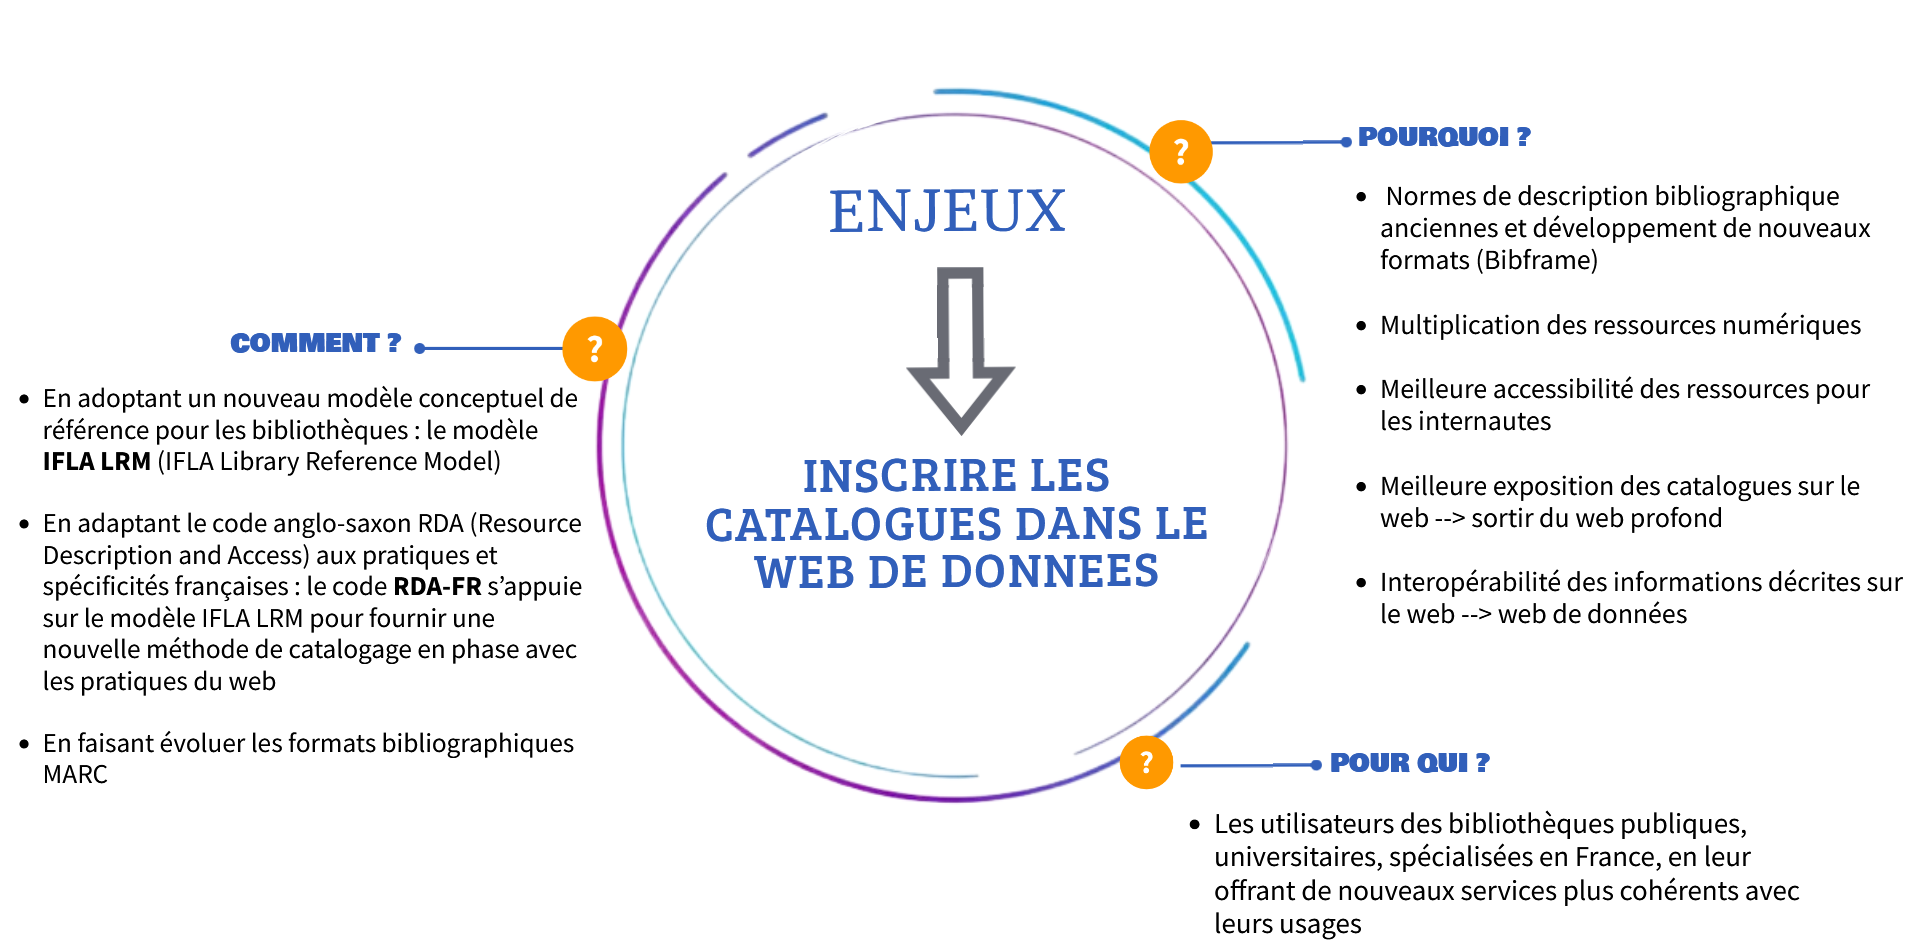
\includegraphics[width=0.8\textwidth]{partie2/images_partie2/images_chapitre5/transition_bibliographique.png}
	\caption{Schéma de la Transition bibliographique (\url{https://www.transition-bibliographique.fr/enjeux/}).}
\end{figure}

Après dix ans de réflexion sur ces normes de formation et de sensibilisation des bibliothécaires, la Transition bibliographique entre dans une phase d’aboutissement et d’implémentation. En témoignent le déploiement de NOEMI, le nouvel outil de catalogage nativement fondé sur les normes LRM et RDA-FR à la BnF, et la préparation du renouvellement du système de gestion des métadonnées de l’Abes.

La Transition bibliographique, dans sa phase d’implémentation, est un enjeu important pour les bibliothèques qui se doivent d’intégrer progressivement ces nouveaux outils dans leur politique documentaire.

\subsubsection*{De la politique documentaire à la gouvernance des données}

Dans un contexte numérique, nous l'avons vu, les bibliothèques expérimentent de nouveaux outils pour mettre en œuvre leur politique documentaire. Pensée non comme le remplacement mais comme le prolongement de la politique documentaire, la gouvernance des données en est un exemple marquant.

La politique documentaire s'articule autour du cycle de vie du document, physique ou numérique, qui se compose en bibliothèque des opérations de sélection, d'acquisition, de traitement, de conservation et de désherbage. Les bibliothèques, dans leur volonté de produire des données structurées, élargissent donc leur politique documentaire à la politique de gouvernance des données.

\begin{quotation}
	La gouvernance des données est la stratégie qui se compose de normes, principes et règles régissant divers types de données au-delà de la gestion purement technique. Elle s'applique à la gestion des données, leur accès, leur stockage, leur mise à jour et leur consommation au sein d’une organisation afin d’en optimiser la valeur et l’efficacité des traitements et des expositions. C'est une stratégie dont le but est d’assurer l’efficacité des traitements liés à la donnée pour assurer son exploitation\footnote{Définition de Lauryne Lemosquet dans le cadre du cours donné aux étudiants de master Technologies Numériques Appliquées à l'Histoire à l'École nationale des chartes.}.
\end{quotation}

La mise en œuvre de la gouvernance des données est un ensemble d'opérations regroupées sous le nom de traitement de la donnée. Comme le document, la donnée a un cycle de vie. Il se compose de la création, du traitement, de l'analyse, de la conservation, de l'accès et de la réutilisation de la donnée\footnote{Voir l'encadré \enquote{Les six étapes du cycle de vie de la donnée}, dans Mesguich (Véronique), \enquote{Chapitre 1. Qu’est-ce qu’une donnée ? Formats, standards, cycle de vie des données…}, \textit{Les bibliothèques face au monde des données}, Villeurbanne, Presses de l’enssib, \url{https://doi.org/10.4000/books.pressesenssib.17761}.}.

Parmi ces opérations, \enquote{l’intégration de la donnée} est une étape clé. Dans le système d’information (SI), les données viennent de sources multiples avec des formats variables. L’opération d’intégration consiste en l’unification de ces sources selon un modèle conceptuel destiné à alimenter des bases de données fiables et interopérables (le \textit{back-end}).

Pour aboutir à cette transition de données brutes à des (méta)données structurées, la démarche d’intégration de la donnée doit répondre à des exigences précises de la gouvernance des données\footnote{Items soulignés par Lauryne Lemosquet dans le cadre du cours donné aux étudiants de master Technologies Numériques Appliquées à l'Histoire à l'École nationale des chartes.} :
\begin{itemize}
	\item \enquote{Un processus de normalisation et de rationalisation orienté vers la qualité}\footnote{\textit{Idem}} ;
	\item \enquote{Une parfaite maîtrise de la sémantique et des règles de gestion des données manipulées}\footnote{\textit{Idem}} ;
	\item \enquote{Une bonne gestion des référentiels, incluant une vérification constante de leur intégrité}\footnote{\textit{Idem}}.
\end{itemize}

Cette politique de gouvernance des données vise à transformer des données à la qualité variable en données traitées et organisées. Dans cette recherche, les référentiels, thésaurus et ontologies constituent un socle sémantique et technique important sur lequel repose l'intégration des données. Si la gouvernance des données ne se limite pas à l'interopérabilité des données, ces outils de référentiels facilitent toutefois l'interopérabilité des données et la mise en œuvre des normes de la politique de gouvernance des données.

\subsubsection*{Référentiels, thésaurus, ontologies : poser les bases de l'interopérabilité}

Les référentiels permettent de poser les fondations de l’interopérabilité. En effet, ils facilitent la cohérence des valeurs attribuées aux métadonnées et garantissent un contrôle du vocabulaire dans les systèmes d’information (SI). Les référentiels sont donc des hubs de données censés connecter les bases de données entre elles au sein d’une même institution ou entre institutions culturelles et patrimoniales différentes.

Pour poursuivre leur objectif d’interopérabilité, les bibliothèques ont recours aux thésaurus, qui sont des outils de structuration. Répondant aux normes internationales ISO 25964-1:2011\footnote{Détails sur la norme ISO 25964-1:2011 : \url{https://www.iso.org/fr/standard/53657.html}.} et ISO 25964-2:2013\footnote{Détails sur la norme ISO 25964-2:2013 : \url{https://www.iso.org/fr/standard/53658.html}.}, les thésaurus fonctionnent ainsi : un concept est exprimé par un terme préféré, les autres termes non descripteurs étant considérés comme des synonymes, par langue. Les concepts sont ensuite reliés à d’autres concepts\footnote{Définition d'Emmanuelle Bermès, donnée dans le cadre d’un cours aux étudiants du master TNAH.}. Un thésaurus s’organise donc selon une modélisation conceptuelle rigoureuse :

\begin{itemize}
	\item \textbf{L’expression univoque des concepts :} chaque concept est exprimé par un (et un seul) terme descripteur par langue (par exemple le concept de \textit{Piano}) ;
	\item \textbf{La gestion des synonymes :} les variantes lexicales, les formes rejetées, les abréviations ainsi que les évolutions chronologiques sont des termes non descripteurs (par exemple, en reprenant le concept de \textit{Piano} : \textit{pianoforte}, \textit{piano à queue}, \textit{Klavier}, \textit{Pno.}) ;
	\item \textbf{Les relations avec d’autres concepts :}
	\begin{itemize}
		\item \textit{Relations hiérarchiques et polyhiérarchiques :} des relations structurées selon des logiques génériques, partitives ou d’instanciation (par exemple la hiérarchie \textit{Instrument de musique} $\gg$ \textit{Instrument à cordes} $\gg$ \textit{Piano}, ou la polyhiérarchie reliant \textit{Instrument à clavier} et \textit{Instrument à cordes frappées} au \textit{Piano}) ;
		\item \textit{Relations associatives :} des relations de liens thématiques, fonctionnels et contextuels (par exemple des liens d'agent/action ou d'association entre \textit{Piano} et des termes techniques associés comme \textit{Pédale douce}, ou encore des noms de marque comme \textit{Steinway \& Sons}).
	\end{itemize}
\end{itemize}

Dans le web sémantique, dont l’objectif est de \enquote{partager, enrichir les données de manière structurée pour donner du sens et améliorer la pertinence des recherches}\footnote{Mesguich (Véronique), \enquote{Chapitre 2. Bibliothèques et web de données}, dans \textit{Les bibliothèques face au monde des données}, Villeurbanne, Presses de l’enssib, 2023, \url{https://doi.org/10.4000/books.pressesenssib.17761}.}, cette structure des thésaurus s’incarne dans le standard SKOS (\textit{Simple Knowledge Organization System}), développé par le W3C (Le World Wide Web Consortium)\footnote{Le W3C élabore des normes et des lignes directrices pour aider chacun à construire et à profiter d’un Web basé sur les principes d’accessibilité, d’internationalisation, de confidentialité et de sécurité : \url{https://www.w3.org/}}. SKOS est le standard permettant de formaliser les thésaurus en graphes exploitables par les machines. Il s’agit d'une ontologie, c’est-à-dire un vocabulaire RDF (\textit{Resource Description Framework}), destinée à décrire des thésaurus. RDF sert à exprimer l’information par des phrases simples appelées triplets. Ces triplets se composent d’un sujet, d’un prédicat et d’un objet :

\begin{itemize}
	\item \textbf{Le sujet :} la ressource décrite, identifiée par une URI (\textit{Uniform Resource Identifier}) ;
	\item \textbf{Le prédicat :} ce qui est dit à propos du sujet (le type de relation qui lie le sujet à l'objet) ;
	\item \textbf{L'objet :} l'entité sur laquelle porte la relation (une autre ressource identifiée par une URI ou une valeur littérale).
\end{itemize}

Dans les triplets, les concepts sont identifiés par des identifiants pérennes comme les URI (\textit{Uniform Resource Identifier}), c'est-à-dire des \enquote{unités de base du web sémantique [qui] sont comme les mots d’un langage [dont RDF serait la grammaire]}. L'ARK (\textit{Archival Resource Key}) est un schéma d'identifiant pérenne (qui s'exprime sous forme d'URI pérenne) utilisé notamment pour les ressources de la BnF afin de citer de façon stable les ressources vers d'autres pages\footnote{Mesguich (Véronique), \enquote{Chapitre 2. Bibliothèques et web de données}, \textit{Les bibliothèques face au monde des données}, Presses de l’enssib, 2023, \url{https://doi.org/10.4000/books.pressesenssib.17741}.}.

Les relations entre concepts sont codifiées par des propriétés précises : \texttt{skos:prefLabel} (terme privilégié), \texttt{skos:altLabel} (synonymes et variantes), \texttt{skos:note} (note d'application précisant le périmètre d'emploi), ainsi que les relations hiérarchiques (\texttt{skos:broader}, \texttt{skos:narrower}) et associatives (\texttt{skos:related}).

Les triplets permettent de transformer l'information en graphe de données. Ainsi, de l'identifiant pérenne à la modélisation de l'ontologie, la gouvernance des données rend la donnée interopérable.

Le standard SKOS modélise les données sous forme de graphe de connaissances, faisant des référentiels des piliers de l’interopérabilité grâce à l’alignement des données.

Le web sémantique distingue principalement deux niveaux de correspondance selon la nature des objets alignés :

\begin{itemize}
	\item \textbf{La propriété d’identité stricte \texttt{owl:sameAs} :} issue de l'ontologie OWL (\textit{Web Ontology Language}, langage standardisé par le W3C pour la formalisation des ontologies), cette propriété affirme une identité stricte entre deux ressources du web désignant la même entité du monde réel ;
	\item \textbf{La propriété d’équivalence \texttt{skos:exactMatch} (ou \texttt{skos:closeMatch}) :} il s’agit d’une relation d’équivalence entre des concepts de thésaurus différents, qui n’affirme pas l’identité stricte des entités.
\end{itemize}

Le projet data.bnf.fr est \enquote{l’un des premiers exemples européens de portail orienté entité}\footnote{Bermès (Emmanuelle), \enquote{Web de données et bibliothèques : l’évolution du modèle d’agrégation des données}, \textit{I2D – Information, données \& documents}, 2016/2 (vol. 53), p. 37, \url{https://www.cairn.info/revue-i2d-information-donnees-et-documents-2016-2-page-37.htm}.}. En utilisant les référentiels, data.bnf.fr regroupe autour de fiches virtuelles (les entités \textit{Auteur}, \textit{Œuvre} et \textit{Thème}) des données dispersées dans différents catalogues (la notice d’autorité, le catalogue général, Gallica) pour attribuer à chaque entité une URI pérenne (un lien ARK).

D’après Emmanuelle Bermès, \enquote{son originalité est de proposer à la fois des pages web destinées aux internautes et des données brutes en RDF reliées avec d’autres jeux de données (DBpedia, VIAF, Europeana, par exemple)}\footnote{Bermès (Emmanuelle), \textit{ibid.}}. Data.bnf.fr peut être vu comme un hub d'entités qui lie ses notices d'autorité (avec la propriété \texttt{owl:sameAs}) à des bases externes (comme Wikidata ou IdRef), tout en s'appuyant sur les propriétés SKOS pour aligner ses langages d'indexation (comme RAMEAU) avec d'autres thésaurus internationaux. Cela permet aux données de la BnF de sortir de leur silo institutionnel pour s'insérer pleinement dans le web de données\footnote{Présentation du projet sur le site officiel de la BnF : \url{https://www.bnf.fr/fr/databnf.fr}.}.

Il apparaît dès lors que la standardisation et l’alignement de ces référentiels constituent des outils indispensables à la constitution d’un web de données patrimoniales.

Pour une plateforme appliquée aux bibliothèques d’orchestre comme LaDocumenta.eu, ce cadre normatif permet d’extraire les collections spécialisées de leurs silos pour les transformer en données de la recherche et de l’interprétation musicale interopérables.




\subsection*{L'interopérabilité des données musicales}

Le web de données aussi appelé\textit{ Linked Open Data} a été décrit par Tim Berners-Lee dans la note \enquote{Linked data\footnote{\url{https://www.w3.org/DesignIssues/LinkedData.html}}} en 2006. Il peut s'entendre comme \enquote{l'application des standards et technologies du web sémantique pour échanger et relier les données structurées sur le web\footnote{Mesguich (Véronique), \enquote{Chapitre 2. Bibliothèques et web de données}, \textit{Les bibliothèques face au monde des données}, Presses de l’enssib, 2023, \url{https://doi.org/10.4000/books.pressesenssib.17741}}}.  Si le web de données permet de sortir les (méta)données des silos applicatifs dans lesquels elles sont cachées, les particularités des documents musicaux conservés en bibliothèques musicales et d'orchestre - comme les conducteurs et les parties séparées, annotés ou non, les imprimés et manuscrits musicaux - peuvent être un frein à l'application des normes traditionnelles de catalogage. 

En effet, les ressources musicales ne sont pas adaptées aux notices bibliographiques standards. Les partitions annotées par exemple présentent la spécificité de se composer à la fois d'un texte musical (notation musicale) et d'annotations, écrites à la main, portant sur l'interprétation ou l'effectif musical (comme des coupures, des coups d'archet...) qui sont fondamentales pour la construction de l'interprétation historiquement informée. Cette particularité de contenir deux typologies d'écritures différentes qui ne peuvent être lues par les mêmes outils complique le traitement de ces ressources. 
En effet, la donnée musicale, qu'elle soit physique ou numérique, donne lieu à de multiples expressions d'une même oeuvre. Le traitement bibliothéconomique d'une telle ressource s'avère compliqué car elle chamboule les règles pré-établies concernant la gestion des collections de la bibliothèque. Que faire si la bibliothèque conserve deux éditions strictement identiques d'une même oeuvre mais annotées par deux chefs différents ? L'annotation pouvant être vue en bibliothéconomie traditionnelle comme une dégradation, quelles motivations peuvent encourager les équipes à garder un tel exemplaire, face au stockage limité en magasin ? Si l'ouvrage est gardé mais n'est pas valorisé dans la plateforme numérique de l'orchestre, quel intérêt si l'annotation n'est pas exploitable d'un point de vue de la recherche ? C'est à ce type de questions que tentent de répondre les initiatives de prises en compte des outils numériques spécialisés dans le traitement de la donnée musicale. 

\subsubsection*{La ressource musicale, une ressource complexe adaptée au modèle orienté entité.}

Dans une bibliothèque d'orchestre, un titre d'oeuvre ne peut pas se résumer en une ressource. Il existe tellement de déclinaisons matérielles d'une même oeuvre qu'il peut s'avérer difficile de les individualiser. Le modèle IFLA-LRM offre alors une solution intéressante pour décrire le plus finement possible les ressources musicales. En effet, le modèle IFLA-LRM permet de séparer de manière rigoureuse \enquote{l'Oeuvre}, \enquote{l'Expression}, \enquote{la Manifestation} et \enquote{l'Item}, c'est-à-dire les quatre entités (OEMI) du modèle IFLA-LRM : 

\begin{itemize}
	\item \textbf{L'Œuvre :} la création abstraite (par exemple la \textit{Symphonie $n^o$ 3 en mi bémol majeur}, op. 55 de Beethoven, \textit{L'éroica}) ;
	\item \textbf{L'Expression :} la réalisation intellectuelle ou artistique spécifique, comme une révision par le compositeur, un arrangement pour orchestre réduit ou une version d'époque (par exemple l'expression orchestrale fixée par la première édition de 1806) ;
	\item \textbf{La Manifestation :} l'édition ou le manuscrit matérialisé sous forme de publication (par exemple  le matériel gravé par Breitkopf \& Härtel) ;
	\item \textbf{L'Item :} l'exemplaire physique annoté, contenant des indications précieuses sur l'interprétation (par exemple le conducteur annoté par Laurence Equilbey, lors de la préparation du concert Beethoven qui aura lieu à la Seine Musicale les 25 et 26 septembre 2026).
\end{itemize}


Ces distinctions d'entités sont très précieuses pour documenter l'interprétation historiquement informée de la musique. En effet, la spécificité des données musicales (par exemple : la \textit{Symphonie $n^o$ 3 en mi bémol majeur}, op. 55 de Beethoven), qui peuvent être à la fois \enquote{Oeuvre}, \enquote{Manifestation} et \enquote{Item}, nécessite une précision importante, voire des outils spécialisés. 
Le chercheur musicologue ou musicien est alors à la recherche d'une interaction sémantique entre l'\enquote{Item} (comme des annotations sur la manière d'interpréter une pièce) et le contexte de l'époque. 
Dès lors, les ontologies du web sémantique comme Doremus (Doing Reusable MUSical data), l'extension FRBRoo(\textit{Functional Requirements for Bibliographic Records} orienté objet)/LRMoo , destinés à la description des catalogues musicaux, permettent de préciser ces relations à l'aide de triplets RDF en spécifiant les liens entre les musiciens, leur instrument, les concerts et la documentation des concerts. 

\subsubsection*{Standards d'encodage musicaux et enjeux de numérisation}

L'interopérabilité des données musicales repose, comme nous l'avons vu, sur le rapport entre les métadonnées de description et le contenu musical décrit. Pour construire cette interopérabilité des données musicales, deux standards existent : 

\begin{itemize}
	\item La\textbf{ MEI }(\textit{Music Encoding Initiative}) est un \enquote{système d'encodage de documents musicaux qui rassemble des spécialistes en musicologie, histoire, humanités numériques ainsi que des bibliothécaires. Ce standard XML permet ainsi aux ordinateurs de lire et reproduire la musique notée\footnote{Feustle (Maristella), Intro to MEI. \url{https://works.hcommons.org/records/vbczn-0af28}}}. La MEI permet d'encoder non seulement la musique notée mais aussi l'apparat critique, les \textit{incipit} et les annotations manuscrites à l'endroit précis, à la note ou à la mesure près. Ainsi, un conducteur numérisé en MEI contient des données de recherche interrogeables par des algorithmes (recherche de motifs mélodiques ...)
	
	\item Le protocole \textbf{IIIF} (\textit{International Image Interoperability Framework}) - à prononcer [trois \enquote{i} F]- est un protocole d'exposition et de manipulation d'images haute-définition qui permet de lier les zones d'une image numérisée (par exemple une annotation de chef sur une mesure précise) avec les structures encodées en MEI ou documentées dans un catalogue de bibliothèque, si la MEI est couplée au standard IIIF-AV (Audio-Visuel), il est possible de lier l'image avec un enregistrement sonore.  
\end{itemize}

\subsubsection*{Référentiels spécialisés en musique et alignements internationaux}

Pour permettre aux fonds musicaux des plateformes musicales numériques à l'image de LaDocumenta.eu d'être interopérables à l'échelle européenne, leur alignement aux grands réservoirs de données est fondamental. 
Ces réservoirs de données, à l'image du RISM ou des thésaurus et autorités spécialisées permettent, comme pour les données non spécialisées, de poser les fondations de l'interopérabilité. 

\begin{itemize}
	\item \textbf{Le RISM (\textit{Répertoire International des Sources Musicales})} est le référentiel mondial de description des sources musicales manuscrites et imprimées.
	
	Les bibliothèques musicales spécialisées peuvent solliciter une demande d'attribution d'identifiant RISM, afin d'avoir une reconnaissance de bibliothèque spécialisée, ou de bibliothèque classique à fonds musical remarquable. Par ailleurs, chaque source musicale inscrite au RISM possède également un identifiant RISM. 
	Ainsi, l'attribution d'un identifiant RISM associée à l'alignement des incipits musicaux au moyen du code Plaine \& Easie\footnote{Le code Plaine \& Easie est un \enquote{système d'encodage de notation musicale conçu pour la capture d'incipits mélodiques : courts fragments de notation musicale qui aident à identifier l'œuvre musicale}. Il est développé et entretenu par le RISM (\url{https://plaine-and-easie.info/}).} permet l'identification numérique d'une source musicale.
 
	\item \textbf{Les thésaurus et autorités spécialisés }: l'alignement des noms de compositeurs, d'instrumentistes et de facteurs d'instruments s'appuie sur des référentiels d'autorité comme la GND (\textit{Gemeinsame Normdatei} de la Bibliothèque nationale allemande) ou VIAF, ainsi que sur des vocabulaires contrôlés d'instruments (tels que le thésaurus de l'MIMO -- \textit{Musical Instrument Museums Online}).
\end{itemize}

En associant le modèle IFLA-LRM, l'encodage du format MEI et la mise en réseau par les triplets RDF, le traitement des fonds musicaux des bibliothèques musicales et d'orchestre érige le matériel d'orchestre en données structurées, réutilisables dans des plateformes numériques de recherche dédiées à la pratique historiquement informée comme LaDocumenta.eu.


\subsection*{Etude de cas : la charte des ressources de LaDocumenta.eu, une réflexion sur l'interopérabilité}

Après avoir détaillé les deux premières parties du livrable de charte des ressources dans le chapitre précédent, nous allons à présent expliquer la dernière partie de ce livrable qui porte davantage sur les particularités numériques et l'interopérabilité. 
\begin{itemize}
	\item La \textbf{troisième partie} du livrable de la charte des ressources de LaDocumenta.eu consiste à décrire et problématiser les particularités d'une plateforme numérique, afin de répondre au sujet même de ce mémoire et de poursuivre la réflexion sur l'exploitation des données des bibliothèques musicales pour la recherche et l'interprétation. La réflexion sur l'interopérabilité des données débute lors de la construction de ce type de plateforme. Les outils de la politique documentaire, à l'instar des chartes des collections, permettent d'expliquer le fonctionnement et les ambitions d'une plateforme en interne, mais aussi à destination du public et de la tutelle des bibliothèques (ici les fonds européens de subvention), et de formaliser la réflexion sur l'interopérabilité. \\ 
	Cette troisième partie est donc le lieu de l'explication des particularités d'une politique documentaire numérique. Elle vise à présenter les choix nécessaires, à la fois méthodologiques et technologiques, au bon fonctionnement d'une telle plateforme. Cette partie s'organise en deux points qui visent à expliquer en quoi la bonne réussite de la plateforme, c'est-à-dire l'accessibilité et la pérennité des ressources, passe par une gestion judicieuse des données, composée de la structuration des données, leur standardisation et les protocoles d'échange. 
	
	\begin{itemize}
		\item Le premier point consiste à décrire le projet LaDocumenta.eu non dans sa mission musicale et documentaire mais d'un point de vue technique. L'entretien mené avec les développeurs a été précieux pour la rédaction de cette section sur la partie technique de la plateforme\footnote[18]{Entretien avec Maxime Touroute, développeur de LaDocumenta.eu, mené le 1er juillet 2026, avec contributions écrites de Marc Karassev, également développeur de LaDocumenta.eu. La grille d'entretien est consultable en annexes (Voir l'\hyperlink{annexe:annexe4entretiendeveloppeur.pdf}{Annexe 4 : Grille d'entretien du développeur.}}).
		
		\item Le deuxième point porte sur les formats et l'interopérabilité de la plateforme LaDocumenta.eu. Il s'agit donc du coeur de ce mémoire, qui propose une réflexion sur l'interopérabilité des données des plateformes numériques musicales pour une exploitation à la fois dans le monde de la recherche et pour les interprétations musicales.
		
		
		Tout d'abord, ce point est le lieu d'un approfondissement sur les infrastructures techniques et les formats de la plateforme. Prémice à la réflexion sur les critères d'admissibilité d'une ressource, ce paragraphe permet de proposer un premier élément de réponse à cette problématique. Ainsi donc, une ressource de LaDocumenta.eu, qu'elle quelle soit,  sera de format PDF, audio ou image, ou alors sera intégré à la plateforme sous la forme d'une intégration de liens URL extérieurs pointant vers des serveurs tiers ou des entrepôts de données institutionnels. 
		LaDocumenta.eu repose donc sur un système de gestion de bases de données relationnelles (SGBDR) PostgreSQL\footnote{Les développements techniques sur les bases de données ont utilisé à profit les cours de Marina Hervieu du master 2 TNAH et leur bibliographie, en particulier : Hainaut (Jean-Luc), \textit{Bases de données. Concepts, utilisation et développement}. 5e édition. Malakoff :Dunod, 2022}, il s'agit du \textit{backend}.
		Cela permet d'avoir une modélisation robuste des entités musicales notamment.  
		Comme nous l'avons vu, en bibliothèque musicale un des éléments les plus importants de la politique documentaire spécialisée en musique est le recours à des référentiels d'auteurs ou de lieux.
		
		C'est pourquoi ce point s'intéresse également aux référentiels d'autorité et à l'alignement des données dans la plateforme pour construire l'interopérabilité. 
		Le catalogage de LaDocumenta.eu s'inscrit dans le web sémantique. La plateforme construit l'interopérabilité de ces données sur des référentiels internationaux comme le RISM, l'ISNI et Geonames.
		
	\end{itemize}
	
\end{itemize}


Ainsi, ce pré-livrable de la charte des ressources, en intégrant les référentiels (RISM, ISNI et Geonames), inscrit le consortium dans la volonté de produire dès le départ un catalogue aligné sur le web de données. 
Nous remarquons que le contrôle des formes de noms et de toponymes ne suffit pas. La structuration des données, au moyen de thésaurus est un prérequis à l'interopérabilité des données de la plateforme. 
Ainsi, la plateforme LaDocumenta.eu aspire à ce que ses ressources soient interrogeables dans d'autres bases et puissent intéragir avec celles-ci, pour s'inscrire dans l'interopérabilité. 
La problématique des référentiels permet alors de clore le chapitre de la politique documentaire en abordant les thématiques de standardisation et d'interopérabilité de la plateforme. Après avoir détaillé la politique documentaire de la plateforme LaDocumenta.eu dans ce premier chapitre, le chapitre suivant s'attellera à présenter les enjeux de la standardisation de données des plateformes numériques dans un objectif de construire l'interopérabilité des données musicales. 	